\documentclass[11pt,letter]{article}
\usepackage[utf8]{inputenc}
\usepackage{amsmath}
\usepackage{amsfonts}
\usepackage{wrapfig}
\usepackage{amssymb}
\usepackage{graphicx}
\usepackage{hyperref}
\usepackage[left=3cm,right=3cm,top=3cm,bottom=2cm]{geometry}
\begin{document}
\pagestyle{empty}
\noindent
\begin{wrapfigure}{r}{0.25\textwidth}
    \centering
    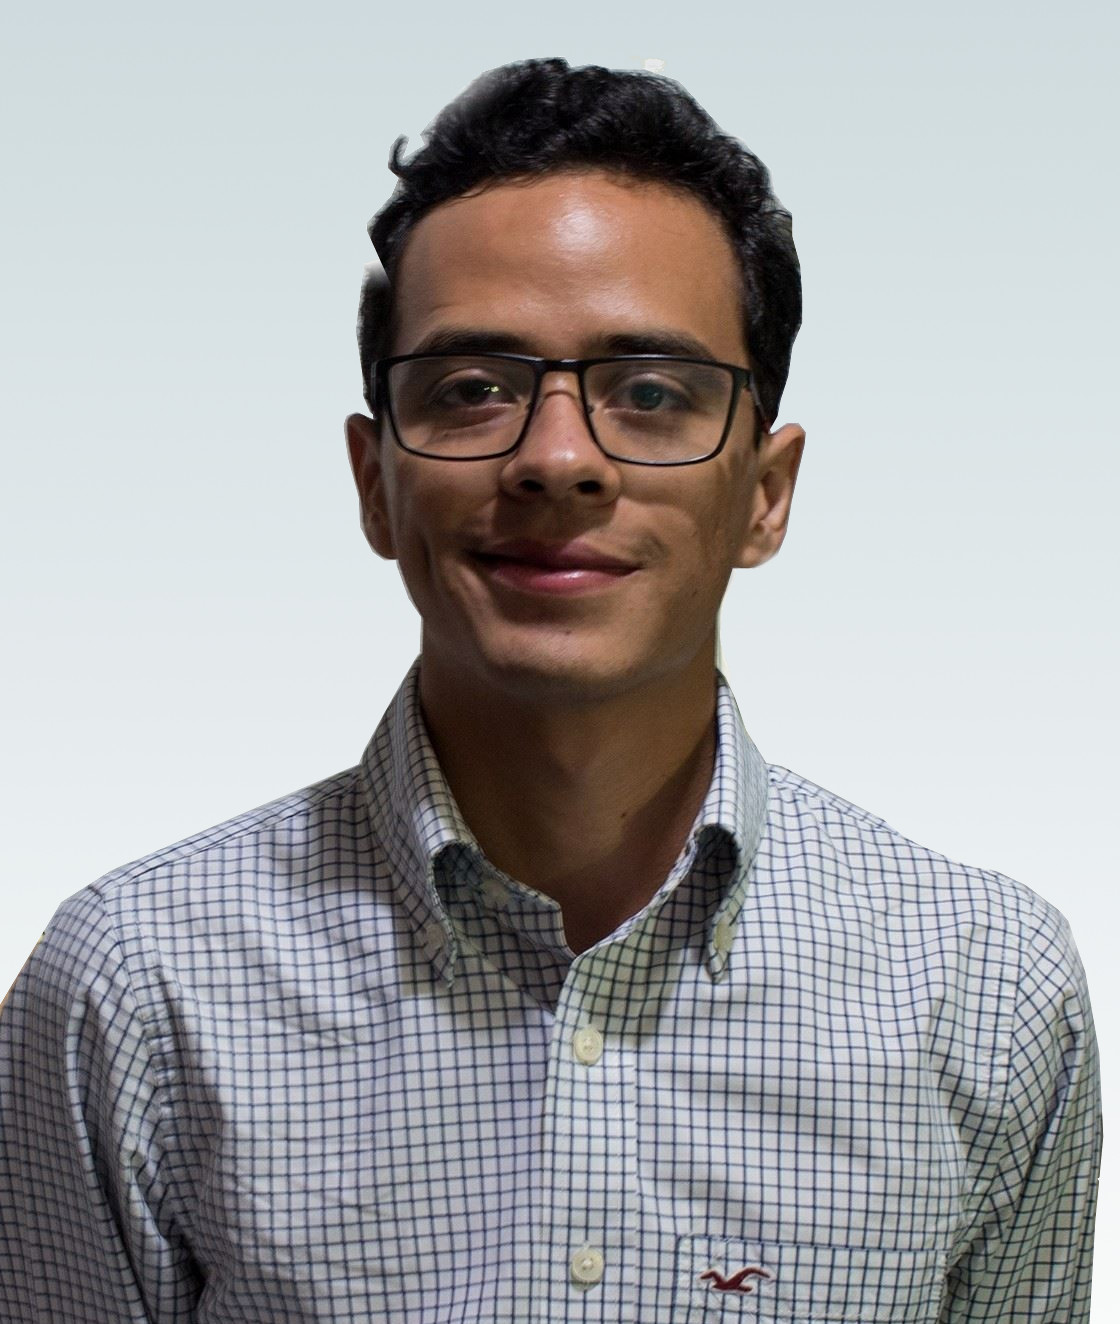
\includegraphics[width=0.2\textwidth]{CV}
\end{wrapfigure} 
\Large{\textbf{Alejandro López Hernández}}  
\\
\normalsize
Villa Federal Mz 13 Lt 6\\ Col. Hank Gonzalez, C.P. 09700, \\Izatapalapa, Ciudad de México, México\\ email: \href{mailto:aleespazx@gmail.com}{aleespazx@gmail.com}\\Tel: 55 40385923 \\ Born 04/02/1996 (22 years old)\\ Personal Blog: \url{http://cienciactuarial.blogspot.mx/}\\\\
\noindent
\textbf{Summary}\\
Actuarial Science student who is interesed in solve real-world problems using statistics and probability as a main tool. I'm developing my skills in measuring risks and programing. My principal motivation is to provide solution to current problematics in the society. \\\\
\textbf{Education}\\
(2014 - Presente) 8th semester of Actuarial Science in Facultad de Estudios Superiores Acatlán (UNAM) with an overall grade of 9.65\\\\
\textbf{Work Experience}\\
(2016 - 2017) \quad Assistant of teacher in the subjects Lineal Algebra I and Lineal Algebra II\\\\
\textbf{Languages}
\begin{itemize}
\item Spanish (Native)
\item Fluid English
\end{itemize}
\textbf{Abilities}
\begin{itemize}
\item Programing in Python (Intermediate)
\item Programing in R (Basic)
\item MS Office Excel
\item SQL (basic)
\end{itemize}
\textbf{Academic Activities}
\begin{itemize}
\item 2017 - Assisted to "Proyecta 10 000 Study Tour" given by MacEwan University in Edmonton, AB, Canada.
\item 2017 - Workshop of creation documents using \LaTeX.
\item 2016 - Assisted to the 4th coloquium of statistics, organized by the Deparment of Mathematics and Enginering at FES Acatlán.
\item 2015 - Took part of the stock exchange simulator, organized by FES Acatlán as a reason of its 40th aniversary.
\item 2014 - Won the contest "Let's Go to San Antonio", and I took a course of English in San Antonio, TX, USA. 
\end{itemize}
\end{document}